\chapter{Contexte et présentation du projet}

\section{Contexte et analyse de l'existant}

\subsection{Contexte}

\subsubsection{Choix des technologies utilisées}
Considérant l'émergence du smartphone ces dernières années et la plus grande accessibilité de \textit{Google} comparé à \textit{Apple} quant à ses mobiles et à ses kits de développement, l'application sera développée sur \textit{Android}. Pour la navigation, l'API \textit{Google} étant mise à disposition pour les développeurs et relativement facile à utiliser, elle s'est vite imposée comme choix d'implémentation. Enfin, l'IDE \textit{Android Studio}\footnote{\url{http://developer.android.com/sdk/index.html}}, supporté par \textit{Google}, a été choisi pour sa complémentarité avec le kit de développement \textit{Android} et ses nombreuses fonctionnalités.\\

\subsubsection{La société \emph{Google}} Filiale depuis 2005 de la société Alphabet en Californie, elle a été créé en 1998 par Larry Page et Sergueï Brin, les créateurs du moteur de recherche éponyme très connu. Elle est devenue au fil des années une des entreprises les plus importantes du Monde, étant celle la plus chèrement cotée en bourse avec une capitalisation boursière de 550 milliards de dollars.\newline
\textit{Google} s'est placé habilement auprès des développeurs par sa contribution à la technologie \underline{Open Source}, lui permettant non seulement de repérer les talents au cours d'événements tel que le \textit{Google Summer of Code}\footnote{\url{https://developers.google.com/open-source/gsoc/?csw=1}}, mais aussi de permettre à la communauté de développer en privé des logiciels sur leur plate-forme, et ainsi de contribuer à la vie de \textit{Google}.

\subsubsection{Le système d'exploitation \emph{Android}} C'est un système d'exploitation mobile basé sur le noyaux Linux, distribué en \underline{Open Source} sous licence Apache\cite{Apache} profitant des services système de base tels que la sécurité, la gestion mémoire ou la gestion de processus.

Le système est organisé en cinq couches: le noyau Linux, les bibliothèques logicielles (OpenGL, WebGL, SQLite,...), un environnement d'exécutions et bibliothèque pour la plate-forme Java, un kit de développement et enfin les applications standards comme un navigateur web, le carnet d'adresses ou l'application de messagerie et de téléphonie mobile.
\textit{Android} bénéficie d'une architecture en couche complète faisant de lui une plateforme riche, dédiée aux appareils mobiles. Depuis le 5 Octobre 2015, les téléphones sont maintenant vendues avec la version 6.0.1 d'\textit{Android}, aussi appelée \textit{Marshmallow}. 

\begin{center}
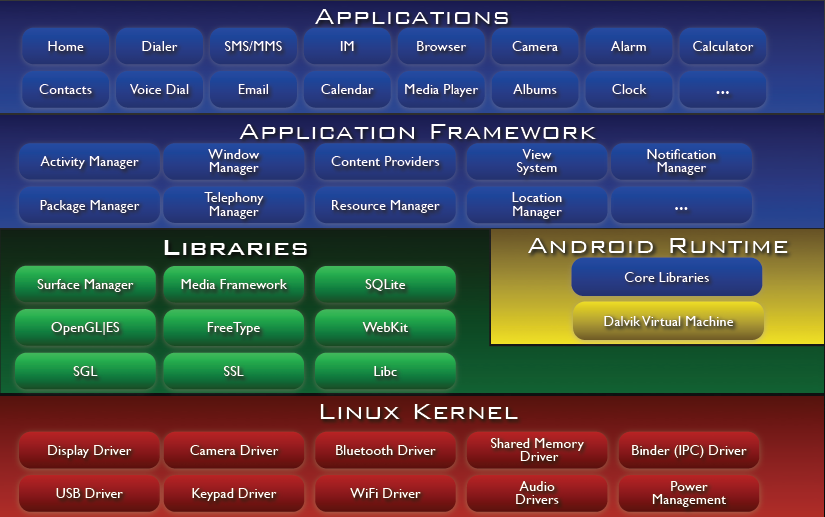
\includegraphics[height=300px]{Assets/androidArchi.png}
\begin{flushleft}
\hspace*{15pt}\hbox{\scriptsize Source:\thinspace{\scriptsize \itshape \url{http://www-igm.univ-mlv.fr/~dr/XPOSE2008/android/archi_comp.html}}}
\end{flushleft}
\captionof{figure}{Architecture Android}

\end{center}

\subsubsection{Fonctionnement d'une application}

Le développement d'une application \textit{Android} se produit au moyen d'un système de compilation automatique, \textit{Gradle} ou \textit{Maven}, qui permettent d'automatiser l'intégration des dépendances. Le langage Java est utilisé, accompagné de multiples extensions intégrées au SDK \textit{Android}, tel que la gestion des activités, leur contexte et l'interaction avec les composants de l'appareil. Le système \textit{Android} fonctionne avec une pile d'activités. Une activité qui se lance est placée en haut de la pile et peut très bien se faire "empiler" par d'autres activités (venant de la même application ou non). Lorsqu'une activité n'est pas au premier plan, elle est soit en pause, soit arrêtée. Ces \underline{activités}, qui composent une application, sont composées de \underline{vues} (éléments graphiques) comportant des \underline{widgets} (boutons, input, etc). L'agencement des éléments graphiques est effectué grâce à des vues spéciales, appelées \underline{layouts}.

\subsubsection{Fonctionnement d'une activité}

\begin{center}
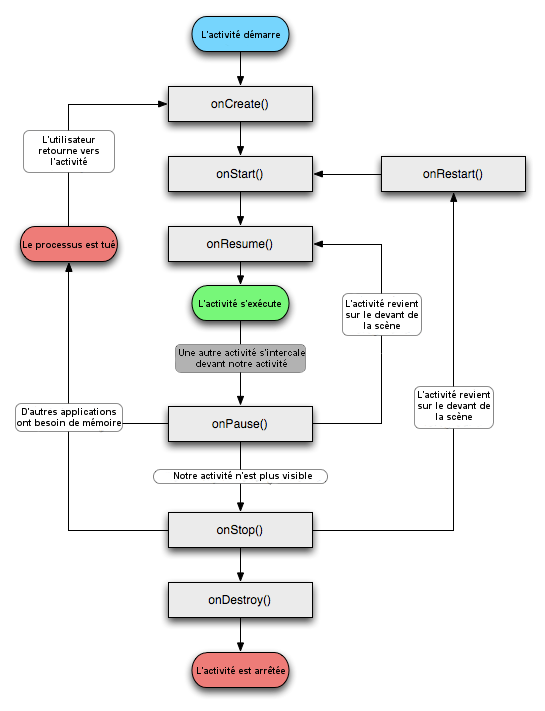
\includegraphics[height=450px]{Assets/cycleActivit_.png}
\begin{flushleft}
\hspace*{15pt}\hbox{\scriptsize Source:\thinspace{\scriptsize \itshape \url{http://developer.android.com/reference/android/app/Activity.html}}}
\end{flushleft}
\captionof{figure}{Cycle de vie d'une activité}

\label{cycleActivité}

\end{center}

Comme représenté sur le schéma, les activités peuvent avoir plusieurs états, et des méthodes de transition sont appelées en entrée et en sortie d'état.
\begin{itemize}
\item onCreate(): permet d'initialiser l'activité, avec en paramètre un objet "Bundle" qui contient des données que l'on peut lui transmettre lorsque l'activité est interrompue (comme lors de la rotation de l'écran).
\item onStart(): appelée ensuite pour charger des données.
\item onResume(): lancée lorsque l'application passe en avant-plan, soit à la première ouverture de l'activité, soit après que la fonction "onPause()" l'ait mise en arrière-plan, en prenant soin d'avoir au préalable sauvegardé l'état de l'activité à renvoyer pour "onResume()".
\item onPause(): appelée lorsque l'activité est "doublée" par une autre activité qui s'affiche par-dessus, l'activité reste affichable.
\item onStop(): intervient lors de la fermeture d'une activité, le processus se met en veille, et il pourra être relancé par la fonction "onRestart()".
\item onDestroy(): la mémoire occupée par l'activité est libérée et l'activité est supprimée de la pile d'activités.
\end{itemize}

\subsubsection{Ressources} Les ressources sont gérées sous \textit{Android} au moyen d'un objet de classe "R" qui permet d'accéder aux fichiers contenant lesdites ressources. Elles sont réparties dans différents dossiers au format XML dans le dossier "/res" du projet. 
\begin{itemize}
\item res/drawable: contient des images au format PNG, JPEG ou GIF, ou des fichiers XML contenant des directives pour dessiner des images.
\item res/layout: contient les fichiers XML décrivant la disposition d'une vue.
\item res/menus: contient les fichiers XML constituant les menus.
\item res/raw: contient des données diverses au format brute, comme des musiques ou des fichiers HTML.
\item res/values: contient diverses ressources telles que des chaînes de caractères, des dimensions, des variables,... 
\end{itemize}

\`{A} l'intérieur de ces dossiers, les ressources sont organisées en sous-dossiers représentant ce que l'on appelle des quantificateurs. Ces quantificateurs divisent ou copient une ressource de sorte quel soit adaptable à une langue ou à un appareil donné, compte tenu des informations présentes dans l'appareil. Ainsi, une application utilisée sur un portable français ira chercher ses ressources "values" dans le dossier "values-fr", et sur un portable anglais dans le dossier "values-en". Il existe divers quantificateurs afin de répartir les ressources en fonction de la taille de l'écran, sa résolution, son orientation ou encore la version de l'API.

\subsubsection{Les layouts}Les \underline{layouts} sont les fichiers XML gérant la disposition des éléments graphiques d'une activité. Ces \underline{layouts} doivent être liés à un objet de classe "Activity" dans la fonction "onCreate()". Ainsi, cette dernière pourra accéder via l'objet "R" aux composants avec lesquelles l'activité doit interagir.

\subsubsection{Le fichier AndroidManifest.xml} Ce fichier, présent pour chaque module, détaille l'ensemble des permissions que le module détient, comme le droit à l'accès au géolocaliseur du téléphone, au vibreur, aux données de l'appareil, mais aussi aux services \textit{Google}. Il contient la description des activités que le module utilisera.\\
Il contient aussi le nom du package du module, la version minimum du kit de développement que le module peut utiliser et les librairies à importer.

\subsection{Analyse de l'existant}

\textit{Google} ainsi que des développeurs indépendants ont déjà produit des applications pour l'accessibilité des personnes malvoyantes à l'évolution mobile, nous devons donc programmer en gardant cela en tête. Nous vous présentons ici quelques applications que les malvoyants peuvent utiliser sur leur téléphone de base, en essayant d'étudier ce que ces applications pourraient nous apporter ou ceux qu'on pourrait leur apporter.

\begin{itemize}
\item \textbf{TalkBack:} Application développée par \textit{Google} qui permet à l'utilisateur de se faire décrire l'écran par une voix synthétique. Cette application change le comportement du téléphone. Par exemple, le fait de cliquer sur une application ou un bouton ne valide pas l'action ciblée, mais sélectionne simplement le widget qui est alors lu par la voix synthétique. Pour valider ce widget ou bouton maintenant sélectionné, l'utilisateur a simplement à cliquer deux fois n'importe où sur l'écran.\\
Cette application qui est disponible de base sur les téléphones nous apporte un moyen de lire nos boutons aux utilisateurs, nous pouvons utiliser cette application en complément. A terme, la lecture de l'écran par une voix synthétique devrait être intégrée à l'application.
\item \textbf{Saisie vocale:} Les smartphones récents ont un microphone et une reconnaissance vocale intégrés, l'utilisateur peut donc utiliser ce moyen de saisie s'il le souhaite. Il est disponible via le bouton représentant un microphone dans le clavier virtuelle de l'appareil, ou par voix en prononçant "OK Google". Cette fonctionnalité native nous permet de ne pas avoir à l'implémenter nous-même.\\
\item \textbf{Navi'Rando\cite{Navirando}:} Dans le domaine du GPS adaptée aux aveugles, il y a \textit{Navi'Rando}, un GPS pour randonneurs malvoyants. Il guide les utilisateurs par une voix synthétique à travers les bois et les montagnes par des chemins préalablement enregistrés par les développeurs dans l'application. Ce codage des chemins "en dur" dans la base de donnée de l'application leur permet d'avoir des informations très précises à propos des obstacles des parcours, et la voix permet de les avertir de chaque obstacle qu'ils vont traverser, leur indiquer la position horaire de cet obstacle.\\
Cette application se rapproche du but de notre projet mais \textit{Navi'Rando} n'est pas un GPS discret, il préconise la précision avant la discrétion alors que nous utiliserons les vibreurs dans un souci de discrétion. De plus, nous utiliserons des itinéraires à déterminer en fonction de plusieurs paramètres, ils ne pourront donc pas être aussi précis que ceux de \textit{Navi'Rando}.
\end{itemize}

\section{Analyse des besoins de l'application}

\subsection{Besoins fonctionnels}

\subsubsection{Choix de l'environnement de programmation} Après quelques tests effectués avec \textit{Android Studio} et \textit{Eclipse} (couplé au plug-in {textit{ADT - Android Development Tools}), les deux semblent convenir pour un bon développement. \textit{Eclipse} est moins lourd à supporter pour certaines machines, mais \textit{Google} ne maintient plus le plug-in sur \textit{Eclipse}\cite{EclipseAndroid}. \textit{Android Studio} est donc utilisé. Ce dernier est développé par \textit{Google} basé sur \textit{IntelliJIDEA}, un des premiers environnements pour \textit{Java}. Il contient des fonctionnalités afin de gérer les fichier XML de layout graphiquement et intègre des outils de compilation comme \textit{Gradle} et \textit{Maven}, afin d'automatiser la création d'une application par une liste de dépendances.

\subsubsection{Android SDK 4.4 Kit-Kat} L'application sera codée en Java, couplé par le XML que nous propose l'architecture d'\textit{Android}. La version 4.4 du kit de développement d'\textit{Android KitKat} sera utilisée, afin que l'application fonctionne sur le plus d'appareils possible. Malgré tout, la version qui sera utilisée pourra en être une autre, mais toujours en préconisant la visibilité de l'application.

\subsubsection{Gestionnaire de versions, SVN} Un gestionnaire de versions va être utilisé afin de disposer d'un dépôt sur le serveur du CREMI mis à disposition aux étudiants. Nous développerons sur une copie de ce dépôt, en local, et nous validerons ces changements lorsque s'ils seront corrects. Le CREMI proposant un serveur SVN, nous utiliserons ce type de gestionnaire qui a l'avantage d'être familier aux étudiants depuis leur entrée dans l'établissement.

\subsubsection{Google Maps API } 
Afin d'utiliser les services de \textit{Google}, il a dû être nécessaire au préalable de se référencer auprès de la société via la console de développeur\footnote{\url{https://developers.google.com/?hl=fr}}. Nous avons donc précisé quel services nous allions utiliser et la console nous a alors transmis une clé d'authentification que nous devons intégrer dans le fichier "manifest" de l'application.
\paragraph{Algorithme d'itinéraire} L'interface de \textit{Google Maps Directions} sera testée. Cette dernière renvoie un fichier sous format JSON décrivant une suite de 23 points maximum (limite standard) constituant l'itinéraire calculé. Un fichier JSON est un fichier de structuration de données basé sur la syntaxe JavaScript. Il permet de représenter des informations sous formes d'arbres, comme le fait XML par exemple. Ce fichier, renvoyé par les services de \textit{Google}, contient tout un tas d'informations décrivant un chemin. Le premier niveau d'information contient les informations globales telles que la durée totale du trajet, le statut de la requête (le nombre d'itinéraires renvoyés, la validation ou non de la requête,...), les points de la ligne graphique à dessiner encodées, les points de cheminements que l'utilisateur veut particulièrement traverser et un ou plusieurs champ "route", représentant un chemin. Ce dernier contient un ou plusieurs "legs", qui eux correspondent aux chemins entre chaque point de cheminement. Ces "legs" contiennent un ou plusieurs champs "step" qui eux représentent les chemins entre chaque mouvement. Ce sont les atomes de ces itinéraires. Ils sont constitués de champs tels que "durée estimée", "prochaine manœuvre" (tourner à gauche par exemple), "point de début et d'arrivé"e et "description du step" au format HTML. Ces données sont à traiter en temps réel afin de se déplacer à travers le fichier JSON en fonction des déplacements de l'utilisateur.
\paragraph{Algorithme de géolocalisation} La géolocalisation a quant à elle une limite standard de 10 requêtes par seconde par utilisateur, dans une limite de 2500 par jour. Elle renvoie un objet de classe "Location" contenant des informations telles que la précision de la réponse, la vitesse de déplacement, la direction (en degré par rapport au Nord), le nom du fournisseur de localisation (par GPS, par WIFI ou par réseau mobile) et bien évidemment la latitude, la longitude et l'altitude du point géographique.

\subsubsection{Matériels} Les émulateurs d'appareils \textit{Android} étant très lents, le client s'engage à fournir des équipements de tests, en l'occurrence des téléphones fonctionnant sous \textit{Android}, afin de travailler dans les meilleurs conditions.\\

\subsubsection{Tests avec JUnit4}
Afin de réaliser les tests de nos fonctionnalités et de nos codes, \textit{Android SDK} fournit un module de test se nommant \textit{JUnit}\footnote{\url{http://developer.android.com/tools/testing/testing_android.html}}, la version 4 sera utilisée pour profiter au mieux du progrès de développement de \textit{JUnit}. 
\paragraph{Tests de régression} Tout les tests seront utilisés au cours du projet afin de vérifier que les nouvelles fonctionnalités apportées ne dérangent pas le bon fonctionnement des précédentes.

\subsection{Besoins non-fonctionnels}
Nous allons présenter dans cette section les besoins non-fonctionnels de l'application par module. Certains aspects expliqués ne sont pas présents dans la version du rendu final, mais nous parlerons plus en profondeur de ces points dans la partie traitant des améliorations possibles.

\subsubsection{Module de saisie d'adresse}
\paragraph{Ergonomie}
L'interface se doit d'être la plus ergonomique possible afin de permettre à un utilisateur malvoyant de naviguer dans les menus avec le plus de facilité possible. Dans l'idéal, chaque item du menu devrait faire l'objet d'une activité qui prendrait tout l'écran, il pourra aussi être envisagé de faire dicter par une boite vocale ce qu'il y a écrit. A chaque changement d'activité, le téléphone vibrera afin de signifier le changement d'activité.

\paragraph{Robustesse et stabilité}
L'ensemble des activités doit être accessible à partir des autres activités, un test doit donc être réalisé sur le graphe des activités pour vérifier qu'il est fortement connexe. Pour tester que l'application ne s'éteint pas prématurément à cause d'un bug, un oracle doit être implémenté. Cet oracle devra aléatoirement se déplaçait dans les activités afin d'augmenter la confiance en la robustesse et la stabilité de l'application.

\subsubsection{Module synchronisation}

\paragraph{Ergonomie}
Pour se synchroniser avec un autre appareil, il faut trouver un moyen efficace et simple qui fournit à un aveugle la possibilité de se connecter en \textit{BlueTooth} sans boîte vocale. Si cela est possible (les possibilités du SDK d'\textit{Android} sont à vérifier), une liste similaire à la liste des adresses devra être implémentée. Cette liste fera figure de surcouche de la boîte de dialogue d'\textit{Android}, permettant à l'utilisateur de choisir avec plus d'ergonomie l'appareil cible. Lorsqu'il aura choisi, l'appareil cible se fera reconnaître de l'utilisateur par une vibration à la demande d'appareillage, de sorte à indiquer à l'utilisateur qu'il doit maintenant appuyer sur l'écran des deux téléphones afin de valider la synchronisation.

\paragraph{Performance} Ils doivent pouvoir recevoir des ondes ou les émettre et ce, d'une rapidité convenable pour simuler un temps réel (estimé à moins d'une seconde de latence).

\paragraph{Batterie} Lorsque la batterie de l'un des deux téléphones se décharge, l'application ne sera plus en mesure de pouvoir guider l'utilisateur puisque la synchronisation sera arrêtée. La vibration sera utilisée pendant trois secondes sur le téléphone non déchargé pour indiquer à l'utilisateur que la synchronisation s'est arrêtée. L'application relancera automatiquement une nouvelle tentative de synchronisation. \emph{La recherche des appareils \textit{BlueTooth} visibles est coûteuse en énergie, elle est à faire le moins possible.}

\paragraph{Sécurité} Du point de vue sécurité, l'application serveur doit empêcher l'utilisateur malvoyant de se connecter par mégarde à un appareil tiers. Une confirmation doit donc être envoyé par le client. Également, l'application client ne doit pas laisser un appareil tiers se connecter à lui.
Les développeurs ne sont pas responsables des accidents qui surviendraient de l'utilisation de l'application sur des téléphones défectueux ou obsolètes qui créeraient des désynchronisations.

\subsubsection{Module de guidage} 
\paragraph{Performances} L'application ne doit pas afficher une localisation qui date de plus d'une seconde en mémoire, afin que le guidage soit le plus fluide possible. Les tests de performances doivent vérifier que, en moins d'une seconde, le téléphone principal reçoit les données de position et les envoie au téléphone secondaire en moins d'une seconde.

\paragraph{Capacité} L'application a un besoin constant de connexion Internet et d'une bande passante convenable qui satisfait les besoins en performance. Ces contraintes sont les mêmes en ce qui concerne la connexion \textit{BlueTooth}.

\paragraph{Disponibilité}
Afin de pouvoir utiliser l'application il est nécessaire d'avoir une connexion Internet, elle est utilisable seulement dans un lieu où le téléphone est susceptible de recevoir les données nécessaires au bon fonctionnement de celle-ci. De plus, l'application ne fonctionnera uniquement dans les lieux qui sont couverts par l'API cartographique de \textit{Google}.

\paragraph{Stabilité du code}
Des tests doivent être fournis qui permettront de certifier la bonne validité du code. 
\subparagraph{Tester les itinéraires} Le module de calcul d'itinéraire doit faire faire l'objet de tests de régression afin de certifier ses résultats.
\subparagraph{Tester les fonctions vibreur} L'application cliente doit vibrer \emph{si et seulement si} l'application serveur est à une intersection et l'itinéraire (certifié) indique la gauche ou que l'utilisateur est en sens inverse. Les mêmes tests sont requis pour l'application serveur. Quand un mauvais chemin est emprunté, les deux applications vibrent de concert un court temps avant de recalculer un itinéraire.

\paragraph{Problèmes envisagés}\subparagraph{} Pour le code à établir pour le vibreur, un simple code pour gauche ou droite ne suffira pas, car une intersection peut avoir plus de 4 routes qui s'y rattachent. Dans le cadre d'un premier prototype, et par concertation avec le client, cette éventualité sera ignorée afin de permettre en premier lieu un guidage par intersection simple.
\subparagraph{} L'application utilisant le vibreur constamment, il faut convenir d'un protocole lorsque le téléphone reçoit un appel, un message, une notification. En d'autres termes, il ne faut pas que le code vibreur soit faussé par une autre application. Là aussi, il est demandé par le client que le premier prototype ne s'occupera pas de ces possibles conflits. 

\paragraph{Sécurité}
Pour un fonctionnement optimal de l'application, l'utilisateur doit donc désactiver toute autre application pouvant utiliser le vibreur. Dans le cas contraire, l'utilisateur s'expose à des conflits qui pourrait mener à des mauvaises indications de direction, et il en sera le seul responsable. \emph{A titre informatif: Deux choix de conception sont possibles: imposer un protocole ou en laisser l'utilisateur le choix en proposant dans les paramètres un menu l'invitant à définir le comportement de l'application pour chaque événement.}

\newpage

\section{Scénarios et diagrammes}

\subsubsection{Diagramme d'états}
\begin{center}
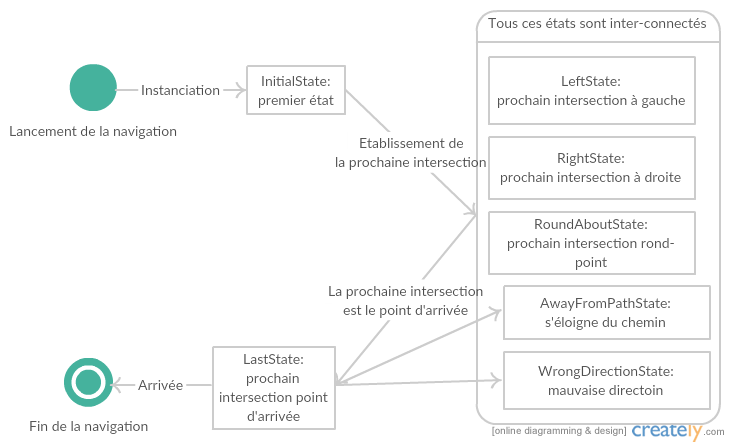
\includegraphics[height=250px]{Assets/State_navigation.png}
\captionof{figure}{Diagramme d'états en navigation}
\end{center}

\subsubsection{Diagramme de Gant}

\begin{figure}[h]
\centering
\caption{Diagramme de Gant prévisionnel}
\label{GantPrévisionel}
\begin{tabular}{llllllllllll}
\cline{1-12}
                                         \diagbox{Tâches}{Semaine} & 5 & 6 & 7 & 8 & 9 & 10 & 11 & 12 & 13 & 14 & 15 \\ \cline{1-12}
Téléchargement des cartes                 & X &   &   &   &   &    &    &    &    &    &    \\
Géolocalisation                           & X & X &   &   &   &    &    &    &    &    &    \\
Calcul d'itinéraires                      &   & X &   & X & X & X  &    &    &    &    &    \\
Mise en place de l'interface              &   & X &   & X & X & X  & X  & X  &    &    &    \\
Test de guidage basique                   &   &   & X &   &   &    & X  &    &    & X  & X  \\
Synchronisation BlueTooth                 &   &   &   & X & X & X  &    &    &    &    &    \\
Mise en place du protocole client/serveur &   &   &   & X & X & X  &    &    &    &    &    \\
Liaison vibreur / application             &   &   &   &   & X & X  & X  &    &    &    &    \\
Persistance des données                   &   &   &   &   &   &    &    & X  & X  &    &    \\
Test de guidage avancée                   &   &   &   &   &   &    &    & X  & X  & X  & X 
\end{tabular}
\end{figure}

%------------------------------

\begin{figure}[h]
\centering
\caption{Diagramme de Gant réel}
\label{GantReel}
\begin{tabular}{llllllllllll}
    \cline{1-12}                                    \diagbox{Tâches}{Semaine} & 5 & 6 & 7 & 8 & 9 & 10 & 11 & 12 & 13 & 14 & 15 \\
    \cline{1-12}
\multicolumn{12}{c}{\textbf{Module Map}}                                                   \\
\cline{1-12}
Téléchargement des cartes                & X &   &   &   &   &    &    &    &    &    &    \\
Géolocalisation                          & X & X &   &   &   &    &    &    &    &    &    \\
Requête d'itinéraire                     &   & X & X & X & X & X  &    &    &    &    &    \\
Gestion des états de navigation          &   &   &   &   &   & X  & X  & X  & X  &    &    \\
Gestion des messages vibratoire          &   &   &   &   &   & X  & X  & X  & X  &  X  &    \\
\cline{1-12}
\multicolumn{12}{c}{\textbf{Module de saisie d'adresse}}                                   \\
\cline{1-12}
Interface graphique 	 				 & X & X & X &   &   &    &    &    & X  & X  &    \\
Utilisation du Geocoder                  &   &   &   & X & X  &   &    &    &    &    &     \\
Base de données							 &   &   &   &   & X &  X &  X &    &    &    &     \\
Vérification de la connectivité réseau	 &   &   &   &   &   &    &    &  X &  X &  X &    \\
Liaison avec les deux autres modules     &   &   &   &   &   &    &    &    &    &  X &    \\ \cline{1-12}
\multicolumn{12}{c}{\textbf{Module de synchronisation}}                                    \\
\cline{1-12}
Communication socket                     &   & X & X & X & X & X  & X  & X  &    &    &    \\
Mise en place du protocole               &   &   & X &   &   &    & X  & X  & X  & X  &    \\
Liaison synchronisation/carte            &   &   &   &   &   &    & X  & X  & X  &    &    \\
Liaison synchronisation/saisie d'adresse &   &   &   &   &   &    &    & X  & X  &    &    \\
\cline{1-12}
\multicolumn{12}{c}{\textbf{Tests}} 
\\
\cline{1-12}
Test module Map							&   &   & X & X & X & X & X & X & X & X & 
	\\
Test module de synchronisation			&   &   &   &   &   &   &   & X & X & X &
\end{tabular}
\end{figure}
\newpage % Sinon l'écriture se met entre les deux tableaux
La différence de ces tableaux est dans la programmation modulaire établie après le diagramme prévisionnel. Tout les modules ont été développés parallèlement et liés entre eux une fois que les fonctionnalités étaient assez développé pour le permettre, en testant au fur et à mesure. 

\subsection{Scénarios possibles}
Pour l'utilisation de notre application, plusieurs scénarios sont possibles. Nous allons nous contenter de décrire deux scénarios possibles avec les différentes étapes.


\textbf{Scénario 1}

1. L'utilisateur démarre l'application et choisit le mode "New Itinerary"

2. L'utilisateur rentre une adresse correcte et celle-ci est enregistrée dans la base de données.

3. L'utilisateur lance l'itinéraire.

4. Le serveur est lancé en arrière-plan et est en attente de connexion entrante.

5. L'itinéraire se dessine sur la carte et la navigation commence.

6. Lorsque l'utilisateur tourne à gauche, deux vibrations sont émises.

7. Lorsque l'utilisateur tourne à droite, une seule vibration est émise.

8. Lorsque l'utilisateur marche tout droit, aucun signalement ne se fait.

9. Lorsque l'utilisateur se trompe dans l'itinéraire, il reçoit  plusieurs vibrations pour l'en avertir. S'il persiste dans la mauvaise direction, un nouvel itinéraire est calculé.

10. Enfin, lorsque l'utilisateur arrive à la destination finale, des vibrations différentes lui indique.

\begin{center}
\captionof{figure}{Diagramme de séquence 1}
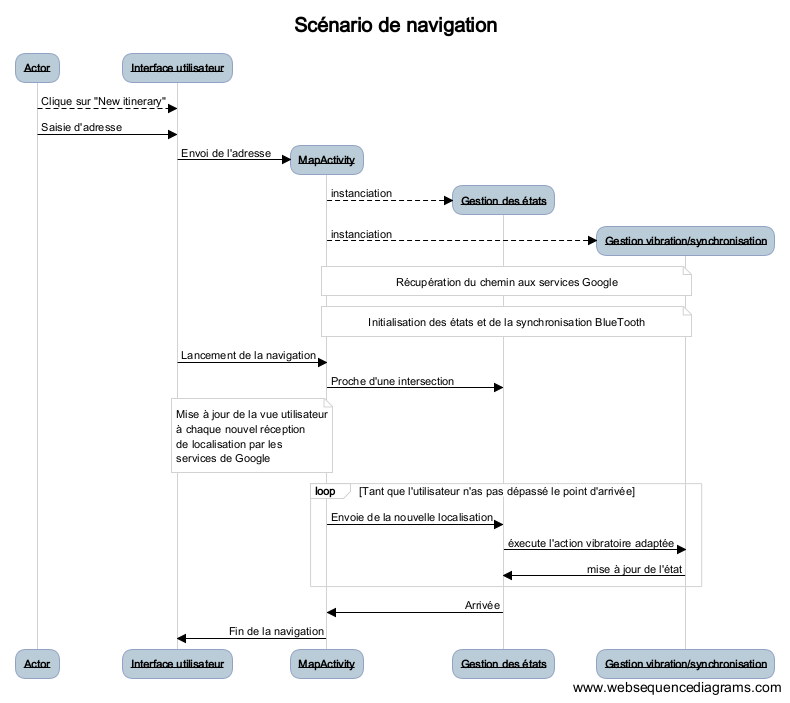
\includegraphics[height=400px]{Assets/scenario1.png}
\end{center}



\textbf{Scénario 2}

1. L'utilisateur possède deux téléphones.

2.L'utilisateur démarre l'application avec le premier téléphone et suit le scénario 1 jusqu'à l'étape 5.

3. L'utilisateur démarre l'application avec le deuxième téléphone et choisit le mode "Launch client".

4. Les deux téléphones font une tentative d'appareillement qui fonctionne.

5. Sur le premier téléphone, le choix du côté pour le lequel le téléphone qu'il tient en main doit vibrer s'affiche. Sur le deuxième téléphone, un message affiche que la connexion s'est bien passée.

6. Le choix de vibration est effectué par l'utilisateur : droite pour le premier téléphone et gauche pour le deuxième.

7. Lorsque l'utilisateur doit tourner à gauche, le deuxième téléphone vibre.

8. Lorsque l'utilisateur doit tourner à droite, le premier téléphone vibre.

9. Lorsque l'utilisateur marche tout droit, aucun signalement ne se fait.

10. Lorsque l'utilisateur se trompe dans l'itinéraire, il reçoit  plusieurs vibrations pour l'en avertir. S'il persiste dans la mauvaise direction, un nouvel itinéraire est calculé.

11. Enfin, lorsque l'utilisateur arrive à la destination finale, des vibrations différentes lui indique.

\begin{center}
\captionof{figure}{Diagramme de séquence 2}
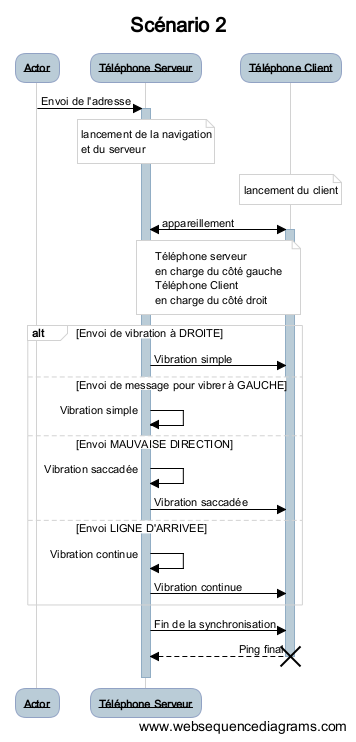
\includegraphics[height=400px]{Assets/scenario2.png}
\end{center}

\textbf{Scénario 3}

1. L'utilisateur suit le scénario 2 jusqu'à l'étape 9.

2. La synchronisation s'arrête car le serveur n'est plus connecté au client.

3. Lorsque le serveur le détecte, il passe directement en mode solo.

4. Le téléphone serveur continue le scénario 1 à partir de l'étape 6. 

\begin{center}
\captionof{figure}{Diagramme de séquence 3}
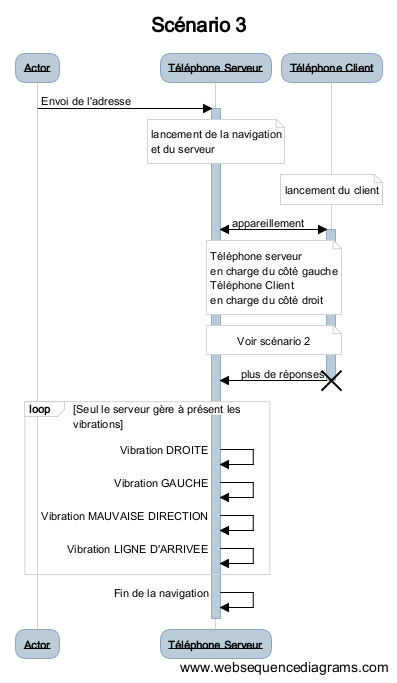
\includegraphics[height=400px]{Assets/scenario3.png}
\end{center}

\textbf{Scénario 4}

1. L'utilisateur suit le scénario 2 jusqu'à l'étape 9.

2. La synchronisation s'arrête car le client n'est plus connecté au serveur. Le client n'a pas reçu d'acquittement du \emph{ping}.

3. Lorsque le client le détecte, il utilise l'adresse qu'il a reçu préalablement du serveur pour continuer l'itinéraire en mode solo. 

\begin{center}
\captionof{figure}{Diagramme de séquence 4}
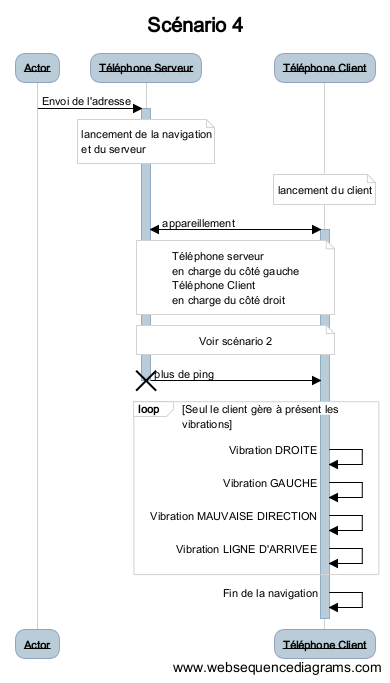
\includegraphics[height=400px]{Assets/scenario4.png}
\end{center}




